\documentclass{beamer}\usepackage[]{graphicx}\usepackage[]{color}
%% maxwidth is the original width if it is less than linewidth
%% otherwise use linewidth (to make sure the graphics do not exceed the margin)
\makeatletter
\def\maxwidth{ %
  \ifdim\Gin@nat@width>\linewidth
    \linewidth
  \else
    \Gin@nat@width
  \fi
}
\makeatother

\definecolor{fgcolor}{rgb}{0.345, 0.345, 0.345}
\newcommand{\hlnum}[1]{\textcolor[rgb]{0.686,0.059,0.569}{#1}}%
\newcommand{\hlstr}[1]{\textcolor[rgb]{0.192,0.494,0.8}{#1}}%
\newcommand{\hlcom}[1]{\textcolor[rgb]{0.678,0.584,0.686}{\textit{#1}}}%
\newcommand{\hlopt}[1]{\textcolor[rgb]{0,0,0}{#1}}%
\newcommand{\hlstd}[1]{\textcolor[rgb]{0.345,0.345,0.345}{#1}}%
\newcommand{\hlkwa}[1]{\textcolor[rgb]{0.161,0.373,0.58}{\textbf{#1}}}%
\newcommand{\hlkwb}[1]{\textcolor[rgb]{0.69,0.353,0.396}{#1}}%
\newcommand{\hlkwc}[1]{\textcolor[rgb]{0.333,0.667,0.333}{#1}}%
\newcommand{\hlkwd}[1]{\textcolor[rgb]{0.737,0.353,0.396}{\textbf{#1}}}%
\let\hlipl\hlkwb

\usepackage{framed}
\makeatletter
\newenvironment{kframe}{%
 \def\at@end@of@kframe{}%
 \ifinner\ifhmode%
  \def\at@end@of@kframe{\end{minipage}}%
  \begin{minipage}{\columnwidth}%
 \fi\fi%
 \def\FrameCommand##1{\hskip\@totalleftmargin \hskip-\fboxsep
 \colorbox{shadecolor}{##1}\hskip-\fboxsep
     % There is no \\@totalrightmargin, so:
     \hskip-\linewidth \hskip-\@totalleftmargin \hskip\columnwidth}%
 \MakeFramed {\advance\hsize-\width
   \@totalleftmargin\z@ \linewidth\hsize
   \@setminipage}}%
 {\par\unskip\endMakeFramed%
 \at@end@of@kframe}
\makeatother

\definecolor{shadecolor}{rgb}{.97, .97, .97}
\definecolor{messagecolor}{rgb}{0, 0, 0}
\definecolor{warningcolor}{rgb}{1, 0, 1}
\definecolor{errorcolor}{rgb}{1, 0, 0}
\newenvironment{knitrout}{}{} % an empty environment to be redefined in TeX

\usepackage{alltt}


% If you have a file called "university-logo-filename.xxx", where xxx
% is a graphic format that can be processed by latex or pdflatex,
% resp., then you can add a logo as follows:
\title{How often does the best team win? A unified approach
to understanding randomness in North American sport}
% \subtitle
% {for Graduate Students} % (optional)
 

%\author[Ofer Harel] % (optional, use only with lots of authors)
%{Ofer Harel\inst{1} and  Gregory Matthews\inst{2}}

\author{Gregory Matthews $^{1}$, Ben Baumer $^{2}$, and Mike Lopez $^{3}$ }



%  \inst{1}
  %Department of Statistics\\
  %University of Connecticut

% - Use the \inst{?} command only if the authors have different
%   affiliation.
\institute [Loyola] % (optional, but mostly needed)
{
  $^{1}$Loyola University Chicago\\
  
  
  $^{2}$Smith College\\
  
  
  $^{3}$Skidmore College\\
  
}



% - Use the \inst command only if there are several affiliations.
% - Keep it simple, no one is interested in your street address.

\date[October 2016] % (optional)
{October, 2016} %Date / Occasion}
\IfFileExists{upquote.sty}{\usepackage{upquote}}{}
\begin{document}
%\SweaveOpts{concordance=TRUE}

\begin{frame}
  \titlepage
\end{frame}

\begin{frame}
  \frametitle{Outline}
  \tableofcontents
  % You might wish to add the option
  % [pausesections]
\end{frame}


\section{Introduction}
%Opening R - some basics (getwd setwd)
%Data Management

\begin{frame}{}
\begin{itemize}
\item Basically everyone who is interested in sports is interested in the question ``Is team $i$ better than team $j$?  
\item How do we measure team strength within a league?
\item If we knew the relative team strengths we could view the outcome as a draw from a random variable with some win probability for team $i$. 
\end{itemize}
\end{frame}

\begin{frame}{}
\begin{itemize}
\item When researchers try to compare sports across leagues, they often use winning percentages.  
\item However, these are problematic.  
\item More sophisiticated techniques have focused on a specific sports. 
\item Hard to compare across sports because of sport specific nuances.  
\item What are the inherent differences in the dispersion and evolution of team strength across sports? 
\end{itemize}
\end{frame}

\begin{frame}{}
\begin{itemize}
\item Instead of estimating win probabilities we work backwards.  
\item We assume that betting markets offer unbiased and low-variance estimates of true probabilities.  
\end{itemize}
\end{frame}


%This manuscript aims to fill these voids. Instead of estimating team strengths within a single sport and using those estimates to generate estimated win probabilities, we work backwards. First, we suppose---and work to validate---that betting market probabilities provide unbiased and low-variance estimates of the true probabilities of wins and losses in each game. Second, using the logit transform of those probabilities, we propose a modified Bayesian state-space model that captures implied team strength and variability. An advantage of this model is that it can be applied uniformly across leagues. Finally, by looking at posterior estimates of within and between season variability, as well as the overall dispersion in team strength estimates, we present unique league-level contrasts which, to this point, have been difficult to capture. As examples, we find that season-to-season reversion to the average is highest in the NHL, and that the gaps in talent in the NBA and NFL overwhelm those of the NHL and MLB.  Additionally, we quantify the relative home advantage for each franchise, as well as between-league differences in the randomness in postseason play. All together, our results better inform an understanding of the dispersion of both talent and randomness in sport. 


\begin{frame}[fragile]
\tiny
% latex table generated in R 3.3.1 by xtable 1.8-2 package
% Wed Oct  5 16:42:40 2016
\begin{table}[ht]
\centering
\begin{tabular}{lrrrrrrr}
  \hline
sport & games & num\_teams & home\_wp & N\_bets & mean\_home\_p & N\_results & coverage \\ 
  \hline
mlb & 21854 &   30 & 0.542 & 21854 & 0.549 & 24299.000 & 0.899 \\ 
  nba & 10781 &   30 & 0.598 & 10781 & 0.619 & 12059.000 & 0.894 \\ 
  nfl & 2294 &   32 & 0.567 & 2294 & 0.590 & 2560.000 & 0.896 \\ 
  nhl & 10535 &   30 & 0.551 & 10535 & 0.566 & 10564.000 & 0.997 \\ 
   \hline
\end{tabular}
\caption{Summary of cross-sport data. Note that we have near total coverage (betting odds for every game) across all four major sports during the 2005--2014 regular seasons.} 
\label{tab:bigfour}
\end{table}

\end{frame}

%Each dot represents a bin of implied probabilities rounded to the nearst hundredth. The size of each dot is proportional to the number of games that lie in that bin. We note that across all four major sports, the observed winning percentages accord with those implied by the betting markets. The dotted diagonal line indicates a completely fair market where probabilities from the betting markets correspond exactly to observed outcomes. In each sport, this diagonal line lies entirely within the standard error surrounding a LOESS regression line, suggesting that an efficient market hypothesis cannot be rejected.
\begin{frame}[fragile]
\begin{knitrout}
\definecolor{shadecolor}{rgb}{0.969, 0.969, 0.969}\color{fgcolor}\begin{figure}
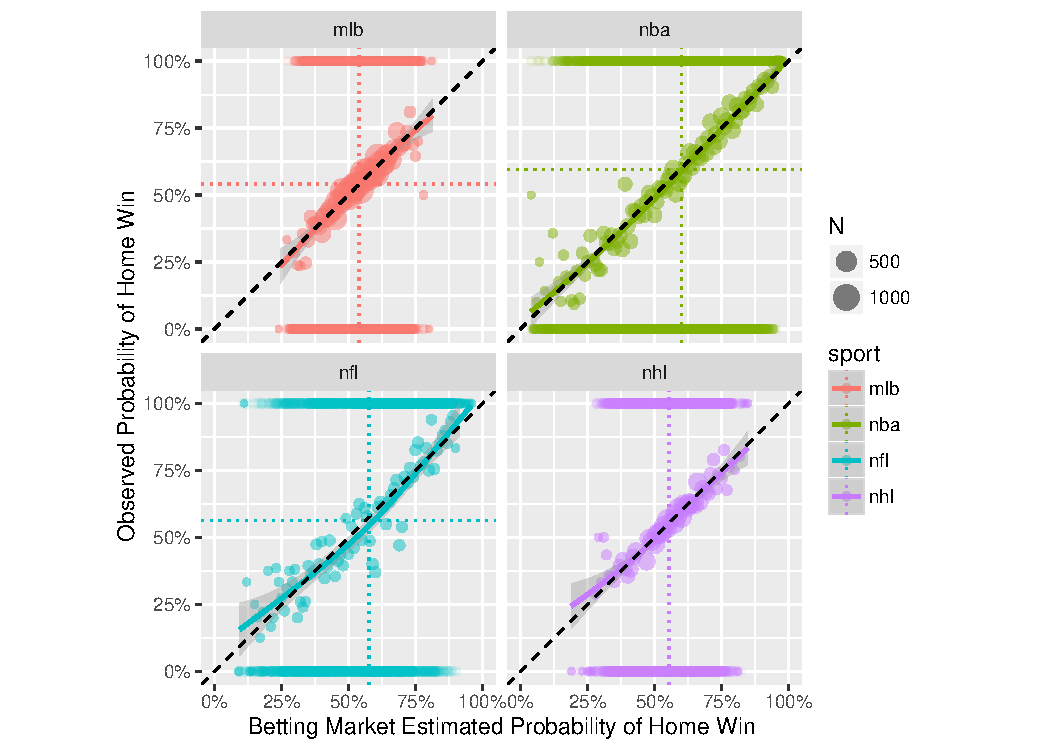
\includegraphics[width=\maxwidth]{figure/betting-1} \caption[Accuracy of probabilities implied by betting markets]{Accuracy of probabilities implied by betting markets. }\label{fig:betting}
\end{figure}


\end{knitrout}
\end{frame}


\begin{frame}
For sport $q$, in season $s$, in week $k$: 
$$
logit(p_{(q,s,k)}) \sim N(\mathbf{\theta_{(q,s,k)}}\mathbf{X}_{q,s,k} + \alpha_{q_0}\mathbf{J}_{g_{q,s,k}} + \mathbf{\alpha}_{q}\mathbf{Z}_{q,s,k}, \tau^{2}_{q,game}\mathbf{I}_{g_{(q,s,k)}}) \,, 
$$

$$
\theta_{(q,s+1,1)} | \gamma_{q,seas}, \mathbf{\theta_{q,s,g_{q,s,.}}}, \tau^{2}_{q,seas},  \sim N (\gamma_{q,seas}\mathbf{\theta}_{(q,s,g_{q,s,.})},(\tau^{2}_{q,seas})I_{t_{q}})
$$
and 
$$
\theta_{(q,s,k+1)} | \gamma_{q,week}, \mathbf{\theta_{q,s,k}}, \tau^{2}_{q,week},  \sim N (\gamma_{q,week}\mathbf{\theta}_{(q,s,k)},(\tau^{2}_{q,week})I_{t_{q}})
$$
\end{frame}

\end{document}




